% !TeX spellcheck = id_ID
\documentclass[a4paper,12pt]{article}
\usepackage[indonesian]{babel}
\usepackage{graphicx}
\usepackage{multirow}
\usepackage{enumitem}
\usepackage{listings}
\usepackage{wrapfig}
\usepackage[T1]{fontenc}
\usepackage{inconsolata}
\usepackage{lipsum}
\usepackage{adjustbox}


\usepackage{color}
\usepackage[table]{xcolor}
\definecolor{mygreen}{rgb}{0,0.6,0}
\definecolor{mygray}{rgb}{0.5,0.5,0.5}
\definecolor{mymauve}{rgb}{0.58,0,0.82}
\lstset{%
    language=java,
    backgroundcolor=\color{white},   % choose the background color
    basicstyle=\footnotesize,        % size of fonts used for the code
    breaklines=true,                 % automatic line breaking only at whitespace
    captionpos=b,                    % sets the caption-position to bottom
    commentstyle=\color{mygreen},    % comment style
    escapeinside={\%*}{*)},          % if you want to add LaTeX within your code
    keywordstyle=\color{blue},       % keyword style
    stringstyle=\color{mymauve},     % string literal style
}

\graphicspath{ {./img/} }
\begin{document}
\title{ {\Large Laporan Praktikum}\\ Algoritma dan Pemrograman Lanjut\\{\Large Pertemuan 1}}

\author{Aldzikri Dwijayanto Prathama 
	\\195410189
	\\Informatika}
\makeatletter
\begin{titlepage}
	\begin{center}
		{\huge \bfseries \@title }\\[14ex]
		
\includegraphics[scale=.8]{logo}\\[4ex]
		{\large \@author}\\[12ex]
		{\large \bfseries {SEKOLAH TINGGI MANAJEMEN INFORMATIKA DAN KOMPUTER
				AKAKOM YOGYAKARTA}}
	\end{center}


%{\large \@date} 
\end{titlepage}
\makeatother
%\maketitle
\newpage
\tableofcontents
\newpage

\section{Tujuan}
\paragraph{}
Mampu memahami dan mengimplementasikan seleksi bertingkat dua dan tiga untuk
menyelesaikan kasus sederhana

\section{Teori}
\paragraph{}
Seleksi sudah dibahas pada Algoritma dan Pemrograman dengan seleksi tunggal dan
ganda. Seleksi digunakan untuk mengarahkan suatu proses itu berjalan. Seleksi adalah
Suatu program untuk mengambil keputusan berdasarkan suatu kondisi. Seleksi ada dua
macam bentuk pernyataan. Seleksi dengan if...else dan switch...case.
Algoritma berbeda dengan bahasa pemrograman (meskipun kadang-kadang syntax-
nya mirip), sebab algoritma memiliki tekanan pada bagaimana cara mendeskripsikan
langkah-langkah yang harus dikerjakan komputer (lebih berkaitan dengan logika/pola pikir
manusia untuk memecahkan masalah tertentu), sedangkan bahasa pemrograman adalah
bahasa yang digunakan – misalnya yang dalam praktikum ini akan digunakan Java – untuk
mengkomunikasikan secara rincian langkah-langkah tersebut pada komputer.
Suatu program komputer yang dibuat menggunakan algoritma tertentu pada umumnya
memiliki perintah-perintah yang hanya akan dikerjakan pada situasi dan kondisi tertentu. Ini
sangat mirip dengan kondisi yang ada di dunia nyata. Di dunia nyata biasanya kita juga
memiliki pilihan-pilihan tertentu untuk melakukan sesuatu (apa yang harus dilakukan/akan
kita kerjakan).

\newpage

\section{Pembahasan}
\subsection{Praktik}
    \begin{enumerate}[label=\textbf{\arabic* .}]
        \item
%%%%%%%%%%%%%%%%%%%%%%%%%%%%%%%%%
    \begin{lstlisting}[frame=single]
import java.util.Scanner;
public class nilai {
    public static void main (String arg[]){
        Scanner in=new Scanner(System.in);
        int nilai;System.out.print("Masukkan angka bulat (0-100) ");
        nilai=in.nextInt();
        if(nilai>=80)
            System.out.println("Nilaimu bagus sekali");
        else if(nilai>=60)
            System.out.println("Nilaimu bagus ");
        else
            System.out.println("Nilaimu kurang ");
    }
}
    \end{lstlisting}
%%%%%%%%%%%%%%%%%%%%%%%%%%%%%%%%%
        Pada program Java di atas terdapat seleksi if, seleksi if pertama memiliki kondisi nilai $>=$ 80, jadi jika variabel nilai dimasukkan angka $>=$ 80, maka program akan menjalankan 
        pernyataan di dalam if. Jika kondisi pada seleksi pertama tidak terpenuhi maka program akan menjalankan seleksi berikutnya yang memiliki kondisi nilai $>=60$, jika kondisi terpenuhi maka
        pernyataan di dalam seleksi ini akan dijalankan, namun jika tidak, program akan menjalankan pernyataan di dalam \texttt{else}\\
        Jika program tersebut dijalankan maka outputnya seperti berikut:\\
            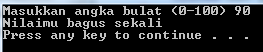
\includegraphics{01b.PNG} 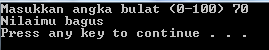
\includegraphics{01c.PNG}
            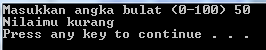
\includegraphics{01d.PNG}

            \newpage
        \item 
%%%%%%%%%%%%%%%%%%%%%%%%%%%%%%%%%
    \begin{lstlisting}[frame=single]
import java.util.Scanner;
public class nilai2{
	public static void main (String arg[]){
        Scanner in=new Scanner(System.in);
        int nilai;
        System.out.print("Masukkan angka bulat (0-100) ");
        nilai=in.nextInt();
        if (nilai>=60){
            if (nilai>=80)
                System.out.println("Nilaimu bagus sekali ");
            else
                System.out.println("Nilaimu bagus ");
        }
        else
            System.out.println("Nilaimu kurang ");
	}
}
            \end{lstlisting}
%%%%%%%%%%%%%%%%%%%%%%%%%%%%%%%%%
        Pada program Java di atas terdapat seleksi if bertingkat, seleksi if pertama memiliki kondisi nilai $>=$ 80, jadi jika variabel nilai dimasukkan angka $>=$ 80,
        maka program akan menjalankan 
        seleksi di dalam if yang memiliki kondisi nilai>=80, jika variabel nilai kurang dari 80, maka program akan menjalankan pernyataan di else. Jika kondisi pada seleksi pertama tidak
        terpenuhi maka program akan menjalankan pernyataan di dalam else\\
        Jika program tersebut dijalankan maka outputnya seperti berikut:\\
            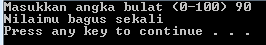
\includegraphics{02b.PNG} 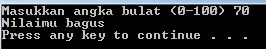
\includegraphics{02c.PNG}
            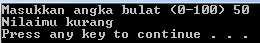
\includegraphics{02d.PNG}

            \newpage
        \item
%%%%%%%%%%%%%%%%%%%%%%%%%%%%%%%%%
            \begin{lstlisting}[frame=single]
import java.util.Scanner;
public class nilai3{
    public static void main (String arg[]){
        Scanner in=new Scanner(System.in);
        int nilai;
        System.out.print("Masukkan angka bulat (0-100) ");
        nilai=in.nextInt();
        if (nilai>=60){
            if (nilai>=80)
                System.out.println("Nilaimu bagus sekali ");
            else
                System.out.println("Nilaimu bagus ");
        }
        else
        {
            if (nilai>=30)
                System.out.println("Nilaimu kurang ");
            else
                System.out.println("Nilaimu jelek ");
        }
    }
}               
            \end{lstlisting}
%%%%%%%%%%%%%%%%%%%%%%%%%%%%%%%%%
            Program diatas memiliki seleksi bertingkat yang berada di dalam if dan else, seleksi pertama memiliki kondisi nilai >= 60, diddalamnya terdapat
            seleksi lagi dengan kondisi >=80.\\
            Sedangkan pada else juga terdapat seleksi, dengan kondisi >=30.\\
            Jika program dijalankan maka outputnya seperti berikut:\\
            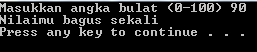
\includegraphics{03b.PNG}
            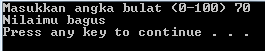
\includegraphics{03c.PNG}
            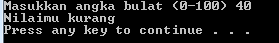
\includegraphics{03d.PNG}
            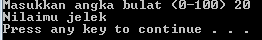
\includegraphics{03e.PNG}

            \newpage

        \item
%%%%%%%%%%%%%%%%%%%%%%%%%%%%%%%%%
            \begin{lstlisting}[frame=single]
import java.util.Scanner;
public class terbesar{
    public static void main (String arg[]){
        Scanner in=new Scanner(System.in);
        int nilai1, nilai2, nilai3;
        System.out.print("Masukkan nilai pertama ");
        nilai1=in.nextInt();
        System.out.print("Masukkan nilai kedua ");
        nilai2=in.nextInt();
        System.out.print("Masukkan nilai ketiga ");
        nilai3=in.nextInt();
        if (nilai1>nilai2){
            if (nilai1>nilai3)
                System.out.println("Nilai terbesar = "+nilai1);
            else
                System.out.println("Nilai terbesar = "+nilai3);
        }
        else {
            if (nilai2>nilai3)
                System.out.println("Nilai terbesar = "+nilai2);
            else
                System.out.println("Nilai terbesar = "+nilai3);
        }
    }
}
            \end{lstlisting}
%%%%%%%%%%%%%%%%%%%%%%%%%%%%%%%%%
            Program di atas adalah program untuk mencari nilai terbesar diantara tiga nilai dengan menggunakan seleksi if. Seleksi if pertama akan membandingkan
            apakah nilai1 lebih besar daripada nilai2, jika benar maka akan kembali dibandingkan nilai3. Jika pada seleksi if pertama tidak terpenuhi maka akan
            masuk ke else, yang mana akan dilakukan perbandingan, apakah nilai2 lebih besar dibanding nilai3.\\
            Jika program dijalankan maka akan seperti berikut:\\
            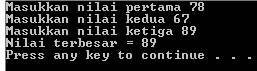
\includegraphics{04b.PNG}

            \newpage
            
        \item 
            \begin{lstlisting}[frame=single]
import java.util.Scanner;
public class terbesar2{
    public static void main (String arg[]){
        Scanner in=new Scanner(System.in);
        int nilai1, nilai2, nilai3;
        System.out.print("Masukkan nilai pertama ");
        nilai1=in.nextInt();
        System.out.print("Masukkan nilai kedua ");
        nilai2=in.nextInt();
        System.out.print("Masukkan nilai ketiga ");
        nilai3=in.nextInt();
        if ((nilai1>nilai2)&&(nilai1>nilai3))
            System.out.println("Nilai terbesar = "+nilai1);
        else if((nilai2>nilai1)&&(nilai2>nilai3))
            System.out.println("Nilai terbesar = "+nilai2);
        else
            System.out.println("Nilai terbesar = "+nilai3);
    }
}               
            \end{lstlisting}
            Program di atas merupakan program sebelumnya yang dimodifikasi dengan menggunakan operator logika \&\& pada kondisi, sehingga dilakukan dua
            perbandingan sekaligur pada setiap kondisi.\\
            Jika program dijalankan maka akan seperti berikut:\\
            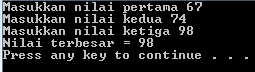
\includegraphics{05b.PNG}

            \newpage

        \item
            \begin{lstlisting}[frame=single]
import java.util.Scanner;
public class spa{
    public static void main (String arg[]){
        Scanner in=new Scanner(System.in);
        int gel;
        String jen,jur;
        System.out.print("masukkan gelombang(1/2): ");
        gel=in.nextInt();
        System.out.print("masukkan jenjang(D3/S1): ");
        jen=in.next();
        System.out.print("masukkan jurusan : ");
        jur=in.next();
        if(gel==1)
        {
            if(jen.equals("D3"))
                System.out.println("SPA gel "+gel+" : Rp. 8.600.000 ");
            else
            {
                if(jur.equals("TI"))
                    System.out.println("SPA gel "+gel+" : Rp. 13.400.000 ");
                else if(jur.equals("SI"))
                    System.out.println("SPA gel "+gel+" : Rp. 12.400.000 ");
                else
                    System.out.println("jurusan tidak terdaftar");
            }
        }
        else if(gel==2)
        {
            if(jen.equals("D3"))
                System.out.println("SPA gel "+gel+" : Rp. 9.100.000 ");
            else
            {
                if(jur.equals("TI"))
                    System.out.println("SPA gel "+gel+" : Rp. 13.900.000 ");
                else if(jur.equals("SI"))
                    System.out.println("SPA gel "+gel+" : Rp. 12.900.000 ");
                else
                    System.out.println("jurusan tidak terdaftar");
            }
        }
        else
            System.out.println("Salah masukkan gelombang");
    }
}               
            \end{lstlisting}
            \paragraph{}
            Program di atas merupakan program untuk menentukan SPA, seleksi tingkat pertama akan menyeleksi gelombang. Kedua seleksi pertama memiliki seleksi if
            di dalamnya yang akan menyeleksi jenjang. Lalu di dalam else terdapat seleksi, yang akan menyeleksi jurusan, dan akan menampilkan SPA yang harus 
            dibayarkan.\\
            Jika program dijalankan maka akan seperti berikut:\\
            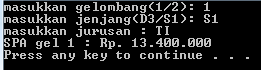
\includegraphics{06b.PNG}

            \newpage

        \item
            \begin{lstlisting}[frame=single]
import java.util.Scanner;
public class spaswitch{
    public static void main (String arg[]){
        Scanner in=new Scanner(System.in);
        int gel;
        String jen,jur;
        System.out.print("masukkan gelombang (1/2/3) : ");
        gel=in.nextInt();
        System.out.print("masukkan jenjang (D3/S1) : ");
        jen=in.next();
        System.out.print("masukkan jurusan : ");
        jur=in.next();
        switch(gel)
        {
            case 1:
            switch(jen)
            {
                case "D3":
                System.out.println("SPA gel "+gel+" : Rp. 8.600.000 ");
                break;
                case "S1":
                switch(jur)
                {
                    case "TI":
                    System.out.println("SPA gel "+gel+" : Rp. 13.400.000 ");
                    break;
                    case "SI":
                    System.out.println("SPA gel "+gel+" : Rp. 12.400.000 ");
                    break;
                    default:
                    System.out.println("jurusan tidak terdaftar");
                }
                break;
            }
            break;
            case 2:
            switch(jen)
            {
                case "D3":
                System.out.println("SPA gel "+gel+" : Rp. 9.100.000 ");
                break;
                case "S1":
                switch(jur)
                {
                    case "TI":
                    System.out.println("SPA gel "+gel+" : Rp. 13.900.000 ");
                    break;
                    case "SI":
                    System.out.println("SPA gel "+gel+" : Rp. 12.900.000 ");
                    break;
                    default:
                    System.out.println("jurusan tidak terdaftar");
                }
            }
            break;
            }
        break;
        default:
        System.out.println("Salah masukkan gelombang");
        }
    }
}
            \end{lstlisting}
            \paragraph{}
            Program tersebut merupakan program sebelumnya yang seleksinya dirubah dari if-else menjadi switch-case. Sama dengan program sebelumnya, switch
            pertama diisi expresi gel, sehingga akan menyeleksi gelombang, lalu switch didalamnya akan menyeleksi jenjang, dan seleksi di dalamnya lagi akan 
            menyeleksi jurusan.\\
            Jika program dijalankan maka akan seperti berikut:\\
            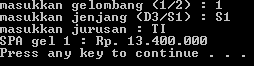
\includegraphics{07b.PNG}

            \newpage

        \item
            \begin{lstlisting}[frame=single]
import java.util.Scanner;
public class spa2{
    public static void main (String arg[]){
        Scanner in=new Scanner(System.in);
        int gel;
        String jen,jur;
        System.out.print("masukkan gelombang(1/2): ");
        gel=in.nextInt();
        System.out.print("masukkan jenjang(D3/S1): ");
        jen=in.next();
        System.out.print("masukkan jurusan : ");
        jur=in.next();
        if(gel==1)
        {
            if(jen.equals("D3"))
            {
                if((jur.equals("TK")) || (jur.equals("MI")) || (jur.equals("KA")))
                    System.out.println("SPA gel "+gel+" : Rp. 8.600.000 ");
                else
                    System.out.println("jurusan tidak terdaftar");
            }
            else if(jen.equals("S1"))
            {
                if(jur.equals("TI"))
                    System.out.println("SPA gel "+gel+" : Rp. 13.400.000 ");
                else if(jur.equals("SI"))
                    System.out.println("SPA gel "+gel+" : Rp. 12.400.000 ");
                else
                    System.out.println("jurusan tidak terdaftar");
            }
        }
        else if(gel==2)
        {
            if(jen.equals("D3"))
                if((jur.equals("TK")) || (jur.equals("MI")) || (jur.equals("KA")))
                {
                    System.out.println("SPA gel "+gel+" : Rp. 9.100.000 ");
                }
            else
                System.out.println("jurusan tidak terdaftar");
            else if(jen.equals("S1"))
            {
                if(jur.equals("TI"))
                    System.out.println("SPA gel "+gel+" : Rp. 13.900.000 ");
                else if(jur.equals("SI"))
                    System.out.println("SPA gel "+gel+" : Rp. 12.900.000 ");
            }
            else
            System.out.println("jurusan tidak terdaftar");
        }
        else
        System.out.println("Salah masukkan gelombang");
    }
}                
            \end{lstlisting}
            \paragraph{}
            Program tersebut merupakan program pada praktik 6 yang sudah dirubah. sehingga, jika dipilih jenjang D3, maka user hanya bisa memilih TK, MI, atau
            KA. Caranya dengan menambahkan seleksi, setelah seleksi if dengan kondisi jen.equals("D3).\\
            Jika program dijalankan maka akan seperti berikut:\\
            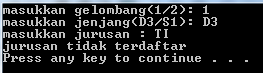
\includegraphics{08b.PNG}

            \newpage

            \item
            \begin{lstlisting}[frame=single]
import java.util.Scanner;
public class spaswitch{
    public static void main (String arg[]){
        Scanner in=new Scanner(System.in);
        int gel;
        String jen,jur;
        System.out.print("masukkan gelombang (1/2/3) : ");
        gel=in.nextInt();
        System.out.print("masukkan jenjang (D3/S1) : ");
        jen=in.next();
        System.out.print("masukkan jurusan : ");
        jur=in.next();
        switch(gel)
        {
            case 1:
            switch(jen)
            {
                case "D3":
                System.out.println("SPA gel "+gel+" : Rp. 8.600.000 ");
                break;
                case "S1":
                switch(jur)
                {
                    case "TI":
                    System.out.println("SPA gel "+gel+" : Rp. 13.400.000 ");
                    break;
                    case "SI":
                    System.out.println("SPA gel "+gel+" : Rp. 12.400.000 ");
                    break;
                    default:
                    System.out.println("jurusan tidak terdaftar");
                }
                break;
            }
            break;
            case 2:
            switch(jen)
            {
                case "D3":
                System.out.println("SPA gel "+gel+" : Rp. 9.100.000 ");
                break;
                case "S1":
                switch(jur)
                {
                    case "TI":
                    System.out.println("SPA gel "+gel+" : Rp. 13.900.000 ");
                    break;
                    case "SI":
                    System.out.println("SPA gel "+gel+" : Rp. 12.900.000 ");
                    break;
                    default:
                    System.out.println("jurusan tidak terdaftar");
                }
            }
            break;
            case 3:
            switch(jen)
            {
                case "D3":
                System.out.println("SPA gel "+gel+" : Rp. 9.600.000 ");
                break;
                case "S1":
                switch(jur)
                {
                    case "TI":
                    System.out.println("SPA gel "+gel+" : Rp. 14.400.000 ");
                    break;
                    case "SI":
                    System.out.println("SPA gel "+gel+" : Rp. 13.400.000 ");
                    break;
                    default:
                    System.out.println("jurusan tidak terdaftar");
                }
                break;
            }
            break;
            default:
            System.out.println("Salah masukkan gelombang");
        }
    }
}
            \end{lstlisting}
            \paragraph{}
            Program di atas merupakan program dari praktik 7, yang sudah ditambahkan dengan gelombang 3. Caranya adalah menambahkan case pada switch pertama, yang memiliki struktur seperti case sebelumnya.\\
            Jika dijalankan maka akan seperti berikut:\\
            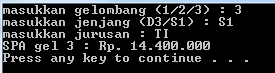
\includegraphics{09b.PNG}
    \end{enumerate}

    \subsection{Latihan}

            \begin{lstlisting}[frame=single]
import java.util.Scanner;
public class Latihan{
    public static void main (String arg[]){
        Scanner in = new Scanner(System.in);
        int jawab;
        System.out.print("1.Mobil 2.Motor = ");
        jawab= in.nextInt();
        switch(jawab)
        {
            case 1:
            System.out.print("1.Honda 2.Suzuki = ");
            jawab = in.nextInt();
            switch(jawab)
            {
                case 1:
                System.out.print("1.Jazz 2.Brio 3.Mobilio = ");
                jawab=in.nextInt();
                switch(jawab)
                {
                    case 1:
                    System.out.println("Jazz = 170jt");
                    break;
                    case 2:
                    System.out.println("Brio = 120jt");
                    break;
                    case 3:
                    System.out.println("Mobilio = 170jt");
                    break;
                }
                break;
                case 2:
                System.out.print("1.APV 2.Swift 3.Ertiga = ");
                jawab=in.nextInt();
                switch(jawab)
                {
                    case 1:
                    System.out.println("APV = 180jt");
                    break;
                    case 2:
                    System.out.println("Swift = 155jt");
                    break;
                    case 3:
                    System.out.println("Ertiga = 160jt");
                    break;
                }
                break;
            }
            break;
            case 2:
            System.out.print("1.Honda 2.Yamaha = ");
            jawab = in.nextInt();
            switch(jawab)
            {
                case 1:
                System.out.print("1.Vario 2.Supra = ");
                jawab=in.nextInt();
                switch(jawab)
                {
                    case 1:
                    System.out.println("Vario = 15jt");
                    break;
                    case 2:
                    System.out.println("Supra = 12jt");
                    break;
                }
                break;
                case 2:
                System.out.print("1.Mio 2.Vixion = ");
                jawab=in.nextInt();
                switch(jawab)
                {
                    case 1:
                    System.out.println("Mio = 14jt");
                    break;
                    case 2:
                    System.out.println("Vixion = 20jt");
                    break;
                }
                break;
            }
            break;
        }
    }
}        
    \end{lstlisting}
    \paragraph{}
    Program diatas merupakan program untuk menampilkan harga mobil dan motor. Seleksi pertama memilih motor atau mobil, lalu seleksi kedua memilih merk motor atau mobil, lalu seleksi terakhir memilih model motor atau mobil.\\
    Jika program dijalankan maka akan seperti berikut:\\
    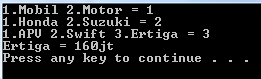
\includegraphics{Latihan3.PNG}

    \newpage
    \section{Kesimpulan}
Setelah praktik ini saya mampu memahami dan mengimplementasikan seleksi bertingkat dua dan tiga untuk
menyelesaikan kasus sederhana

\end{document}
